\section{Regelungskonzepte basierend auf Methoden des maschinellen Lernens}

In Abschnitt \ref{cha:regelung} ist bereits das allgemeine Regelungskonzept vorgestellt worden. Nachfolgend erfolgte eine Reihe von Erläuterung über verschiedene Typen von neuronalen Netzen, welche in der Lage sind, dynamische Nichtlinearitäten eines System durch die Adaption der Gewichte zu approximieren bzw. zu lernen. Nun ist es denkbar, auf Basis neuronaler Netze ein Blackbox-Modell eines nichtlinearen dynamischen Systems zu entwickeln, welches entweder als Hilfsglied in einem Regelkreis oder direkt als Regler fungiert. Dafür sind verschiedene Regelungskonzepte in der Literatur gegenwärtig. Es erfolgt nun eine Übersicht der Regelungskonzepte aus Basis der Methoden des maschinellen Lernens in den Kategorien \textit{überwachtes} und \textit{bestärkendes Lernen}.\\


\subsection{Überwachtes Lernen} 

Im Bereich des \textit{überwachten Lernens} gibt es eine Reihe von verschiedenen Regelungskonzepten auf Basis neuronaler Netze, für die nun ein Überblick gegeben wird.


\subsubsection{Direkte inverse Regelung}
\label{cha:direct_inverse}
Das von \cite{Werbos.2014} erstmals eingeführte Regelungskonzept der \textit{direkten inversen Regelung} basiert auf der Annahme, dass für ein dynamisches System eine inverse Abbildung des Ausgangszustandes in den Eingangszustand existiert.  Ist dies der Fall, kann ein neuronales Netz offline, also nicht während der Betriebseinsatzes, so trainiert werden, dass es die inverse Dynamik der Regelstrecke (in Abbildung \ref{fig:direct_inverse_offline} als Roboter bezeichnet) abbildet. \\ 

\begin{figure} [h]
	\centering
	\includegraphics[width=0.75\textwidth]{images/direct_inverse_control_offline}
	\caption{Direkte inverse Regelung mit offline-Netztraining \cite{Sklyarenko.2002}}
	\label{fig:direct_inverse_offline}
\end{figure}

Daraufhin ist eine direkte Schaltung der neuronalen Netzes in den Regelkreis möglich.  In der Regel findet dann eine Übergabe der Sollgröße $r$ an das invertierte neuronale Netz statt, siehe auch \cite{Almusawi.2016}. Die Ausgangsgröße des neuronalen Netzes entspricht dann den Stellgrößen der Regelstrecke.  Entsprechen die Ausgangsgrößen der Regelstrecke $y$ nicht im ausreichenden Maße den Sollgrößen $r$, ist es zweckmäßig, das Netz offline erneut zu trainieren. Jedoch findet während des Betriebes keine direkte Fehlerrückführung statt, sodass eine stabile Regelstrecke Voraussetzung ist. Offline trainierte Netze gehören zur Klasse der nicht adaptiven Regler.   \\
Beim Konzept der \textit{direkten inversen Regelung} ist es auch möglich, die Adaption der Netzwerkgewichte während des Betriebes, also online, vorzunehmen, siehe Abbildung \ref{fig:direct_inverse_online}. 

\begin{figure} [h]
	\centering
	\includegraphics[width=0.75\textwidth]{images/direct_inverse_control_online}
	\caption{Direkte inverse Regelung mit online-Netztraining \cite{Sklyarenko.2002}}
	\label{fig:direct_inverse_online}
\end{figure}

Diese Regler gehören zur Klasse der adaptiven Regler, da eine Anpassung der Regelparameter während des Betriebs stattfindet. Dabei soll das Netz möglichst den Fehler $e_c$ minimieren, was jedoch nicht immer möglich ist, da die Jacobi-Matrix des nichtlinearen dynamischen Regelstrecke in der Regel nicht bekannt ist. Die Kenntnis der Jacobi-Matrix ist allerdings für Minimierung der Fehlerfunktion unabdingbar. Nach \cite{Sklyarenko.2002} ist es jedoch möglich, die Elemente der Jacobi-Matrix numerisch mit einer Differenzengleichung zu ermitteln. Ein weiterer Nachteil ergibt sich dadurch, dass die Regelstrecke anfangs mit einem untrainierten neuronalen Netz betrieben wird, was zu unkontrolliertem Systemverhalten führen kann. \\

Häufig kommen \textit{inverse neuronale} Regler in Kombination mit anderen Reglern zum Einsatz. Beispielsweise nutzt \cite{Miller.1989} ein neuronales Netz in Kombination mit einem P-Regler zur Steuerung eines Industrieroboters. \cite{Nordgren.1993} und \cite{Jung.1995} kombinieren ein \textit{inverses neuronales} Netz mit einem PD-Regler zur Regelung eines gekoppelten Pendelsystems und zur Regelung eines Industrieroboters. \cite{Andersen.1990} dagegen nutzt einen PID-Regler in Kombination mit einem neuronalen Netz, um die optimalen Schweißparameter beim Lichtbogenschweißen zu ermitteln.   


\subsubsection{Indirekte neuronale Regelung mit Referenzmodell}

Wie in Abschnitt \ref{cha:direct_inverse} erläutert, stellt sich bei der \textit{direkten inversen} neuronalen Regelung das Problem, dass in vielen regelungstechnischen Anwendungen die Jakobi-Matrix der dynamischen nichtlinearen Regelstrecke nicht bekannt ist. Damit gestaltet sich die Gewichtsadaptierung des inversen neuronalen Netzes als schwierig, um die Differenz zwischen der Ausgangsgröße des dynamischen Systems $y$ und der Sollgröße $r$ zu minimieren. Dieses Problem umgeht die indirekte neuronale Regelung mit Referenzmodell, siehe Abbildung \ref{fig:indirect_control}.


\begin{figure} [h]
	\centering
	\includegraphics[width=0.75\textwidth]{images/indirect_control}
	\caption{Indirekte neuronale Regelung mit Referenzmodell \cite{Sklyarenko.2002}}
	\label{fig:indirect_control}
\end{figure}

Im Unterschied zur \textit{direkten inversen} neuronalen Regelung ist ebenfalls ein nicht invertiertes neuronales Netz Bestandteil der Regelstruktur (in Abbildung als NM bezeichnet), siehe \cite{Nguyen.1990}, \cite{BenNasr.2014} und \cite{HUSSAIN.1999}. Dieses ist derartig offline trainiert, dass es die Eingangsgröße der Regelstrecke $u$ in die  Ausgangsgröße $y$ der Regelstrecke transformiert. Während des Betriebs findet keine Gewichtsadaptierung des Netzes NM mehr statt, da dieses nun als Referenzmodell dient. Dagegen findet die Gewichtsadaptierung des Netzes NC während des Betriebes (online) derartig statt, dass die Differenz zwischen der Ausgangsgröße des Netzes NM $\hat{y}$ und der Sollgröße $r$ minimiert wird. Dies ist deshalb möglich, da der Fehler $e_c$ durch das bekannte Netz NM hindurch propagiert (z.B. durch den Backpropagation-Algorithmus) werden kann. Die Regelgüte dieser Regelstruktur hängt sehr stark von der Approximationsfähigkeit des NM-Netzes in Bezug auf die aktuelle Regelstrecke ab. Kommt es im Laufe der Zeit zu Veränderungen in Bezug auf das dynamische Verhalten der Regelstrecke, muss das NM-Netz neu trainiert werden, um es an das aktuelle Verhalten der Regelstrecke anzupassen.  Zudem gibt es keine Rückführung des Fehlers $e_m$, welcher die Differenz zwischen dem realen Systemausgang $y$ und der Sollgröße $r$ abbildet. Die Stabilität dieser Regelstruktur ist in \cite{VijayaKumar.2009} und \cite{Ruan.2007} diskutiert.
 

\subsubsection{Internal Model Control (IMC)}

Wie im letzten Abschnitt erwähnt, findet bei der \textit{indirekten neuronalen Regelung mit Referenzmodell} keine Rückführung des Fehlers $e_m$ statt. Davon unterscheidet sich die IMC-Regelstruktur, da hier der Fehler $e_m$ als zusätzliche Eingangsgröße für das Netz NC dient, siehe Abbildung \ref{fig:imc}.


\begin{figure} [h]
	\centering
	\includegraphics[width=0.75\textwidth]{images/imc}
	\caption{Internal Model Control-Regelkreis \cite{Sklyarenko.2002}}
	\label{fig:imc}
\end{figure}

Wie bei der \textit{indirekten neuronalen Regelung mit Referenzmodell} kommt das invertierte Netz NC zum Einsatz, welches die Stellgrößen $u$ für die Regelstrecke vorgibt. Das offline trainierte Netz NM dient wieder als Referenzmodell und generiert die Ausgangsgröße $\hat{y}$. Die Gewichtsadaptierung des Netzes NC findet nun derartig statt, dass der Fehler $e_c$, welcher die Differenz zwischen der Sollgröße $r$ und der Ausgangsgröße $\hat{y}$ abbildet, minimiert wird. Dies ist möglich, da der Fehler durch die bekannte Netzstruktur NM propagiert werden kann. Nach \cite{Kambhampati.2000} ist es üblich, bei IMC-Regelstrukturen Filter zur Erhöhung der Robustheit einzusetzen. Zudem diskutiert \cite{Kambhampati.2000} den Stabilitätsnachweis und die Auswirkungen der Auswahl von Netzstrukturen (Feed-Forward vs. rekurrentes Netz) bei IMC-Regelkreisen. 


\subsubsection{Feedback Linearisierung mit neuronalen Netzen}

Die Grundidee beim Verwenden linearisierter neuronaler Modelle besteht darin, nichtlineare Systeme für einen bestimmten Arbeitspunkt in lineare Modelle zu transformieren. Zunächst findet das Training eines neuronalen Netzes derartig statt, dass es die Dynamik der Regelstrecke abbildet. Daraufhin findet die Linearisierung des Modells bei einem bestimmten Arbeitspunkt statt, sodass das diskrete Modell durch

\begin{equation} 
y(k+d) = f(\textbf{y},\textbf{u}) + b(\textbf{y},\textbf{u}) \cdot u(k+1)
\end{equation}

mit $\textbf{y} = [y(k), y(k-1), ... , y(k-n+1)]^{T}$ als diskreter Zustandsvektor,          $\textbf{u} = [u(k), u(k-1),... ,u(k-m+1)]^{T}$ als diskreter Stellgrößenvektor und $b(\textbf{y},\textbf{u})$ als weiterer diskreter Zustandsvektor beschrieben ist.
Daraufhin kann die Stellgröße des nächsten Zeitschrittes $u(k+1)$ nach \cite{Mohammadzaheri.2012} durch 

\begin{equation} 
u(k+1) = \frac{y_d(k+d) - f(\textbf{y},\textbf{u})}{b(\textbf{y},\textbf{u})}
\end{equation}

ermittelt werden. Diese führt dazu, dass die Zustandsgröße $y(k+d)$ gegen die Sollgröße $y_d(k+d)$ konvergiert. Dabei approximiert das neuronale Netz die Funktionen \textit{f} und \textit{b}. Die Übergabe der Stellgröße $u(k+1)$ kann dann durch einen vorher trainierten linearen Regler an die Regelstrecke stattfinden, siehe Abbildung \ref{fig:linear}. 

\begin{figure} [H]
	\centering
	\includegraphics[width=0.65\textwidth]{images/linear}
	\caption{Feedback Linearisierung mit neuronalen Netzen \cite{Sklyarenko.2002}}
	\label{fig:linear}
\end{figure}


Das neuronale Netz ist also nicht direkt als Regler, sondern als Hilfsglied für den Entwurf bzw. Training des linearen Reglers verantwortlich. Die Bezeichnung der auf diesem Prinzip basierenden Regelsysteme lautet \textit{NARMA-L2-Control}. Bei dieser Methode kommen sowohl MLP- \cite{Leeghim.2008} als auch RBF-Netze \cite{Deng.2008} zum Einsatz. Nach \cite{Leeghim.2008} kann sowohl eine Änderung des Regelgesetzes während des Betriebs (adaptive Regelung) als auch die Stabilität solcher Regelkonzepte nachgewiesen werden.


\subsubsection{Neuronale prädiktive Regelung}


Prädikative Regelungen verwenden neuronale Netze, um die Ausgangsgröße der Regelstrecke für einen zukünftigen Zeithorizont zu prädizieren, siehe Abbildung \ref{fig:predictive}.


\begin{figure} [h]
	\centering
	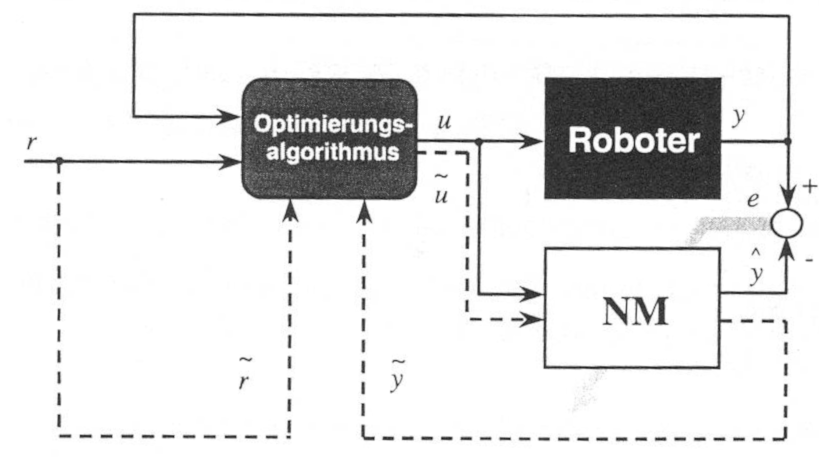
\includegraphics[width=0.65\textwidth]{images/predictive}
	\caption{Neuronale prädiktive Regelung \cite{Sklyarenko.2002}}
	\label{fig:predictive}
\end{figure}




Dabei ist das neuronale Netz derartig trainiert, dass es die Eingangsgröße $u(k)$ der Regelstrecke in die zukünftige Ausgangsgröße $y(k+n)$ transformiert. Nach dem Training prädiziert das neuronale Netz die Ausgangsgröße $\hat{y}(k+n)$ über $n$ Zeitschritte hinweg. Nach der Prädiktion  kommt eine Fehlerfunktion zum Einsatz, welche üblicherweise die Prädiktionsfehler und die Veränderung der Eingangsgrößen berücksichtigt. Abschließend minimiert ein Optimierungsalgorithmus die bekannte Fehlerfunktion. 

Bei prädiktiven neuronalen Regelungen kommen in der Regel MLP- \cite{Mohammadzaheri.2010}, RFB- \cite{Alexandridis.2005} und Neuro-Fuzzy-Netzwerke \cite{Liu.2006} zum Einsatz. \cite{Parlos.2001} und \cite{Alexandridis.2005} trainierten die Netze online (während des Betriebsprozesses), sodass hier von adaptiven prädiktiven neuronalen Netzen gesprochen werden kann. Zudem passte \cite{Parlos.2001} die Modellstruktur und das Regelgesetz so an, dass stabile Regelkreise entstehen. Als Optimierungsalgorithmen kommen unter anderem der Levenberg-Marquardt \cite{Mohammadzaheri.2010}- und der Fuzzy-Gradienten-Algorithmus zum Einsatz. Weitere Beispiele sind der lineare quadratische Gaußsche-Regler \cite{KKaramodin.2009} und das sequentielle quadratische Programmieren \cite{Prasad.1998} \cite{Parlos.2001}. Auch neuronale Netze können als Optimierer fungieren \cite{KOKER.2006}.

\subsubsection{Regelungssysteme mit neuronalen Netzen als Kompensatoren}

Häufig kommen neuronale Netze nicht als Regler, sondern als Hilfsglieder in Regelkreisen zum Einsatz, um Unsicherheiten dynamischer Systeme zu kompensieren. Dafür ist eine Zerlegung des Systems in der Zustandsraumdarstellung in bekannte und nicht bekannte Funktionen zweckmäßig. Die unbekannte Funktion ist von dem Zustandsvektor und dem Stellgrößenvektor abhängig und repräsentiert die Unsicherheiten des dynamischen Systems. Häufig kann dann ein Regelgesetz aufgestellt werden, in welchem die unbekannte Funktion durch ein neuronales Netz approximiert werden kann. Dadurch ergibt sich dann eine Stellgröße, welches die Unsicherheit des dynamischen Systems mit berücksichtigt bzw. kompensiert. In solchen hybriden Regelsystemen kommen neuronale Netze in Kombination mit P- \cite{Ren.2009}, PID- \cite{Hong.2009}, Sliding Mode- \cite{Han.2009}, Back-Stepping- \cite{Jolly.2009}, Feedback Linearisierungs- \cite{Yang.2007} und Modell-Referenz-Reglern \cite{Zhao.2009} zum Einsatz. Dabei finden häufig MLP- \cite{Cheng.2009}, RFB- \cite{Yang.2007}, Neuro-Fuzzy- \cite{Han.2009}, Sigma-Pi- \cite{Hong.2009} und Wavelet-basierte neuronale Netze \cite{Hsu.2009} Anwendung.






